%=========================================================
%  JTAG/cJTAG Debugger Interface for OpenOCD
%=========================================================
\section{JTAG/cJTAG Debugger Interface for OpenOCD}

%=========================================================
\subsection{USB to JTAG/cJTAG Interface for OpenOCD}

The commercial Olimex ARM-USB-OCD(H) is one of the recommended JTAG/cJTAG Debugger interfaces for OpenOCD. However, you can make an almost-compatible one by using the FTDI FT2232D chip. To do so, the commercial breakout board of FT2232D is convenient. You can get the board from the following URL.\\
\texttt{https://akizukidenshi.com/catalog/g/gM-02990/}\\
 Figure \ref{fig:USBJTAGOUTLINE} shows the outline of the interface board. The left one is a convenient version made with a breadboard and the breakout board of FT2232D. The right one is made with a printed-circuit board and the breakout board.

\textit{NOTE: If you use the breakout board of FT2232D shown above, please set the jumper pins as follows: JP1=short, JP2A=open, and JP2B=open, in order to supply 3.3V to VCCIOA and VCCIOB of the FT2232D chip from the target FPGA board.}

\begin{figure}[H]
    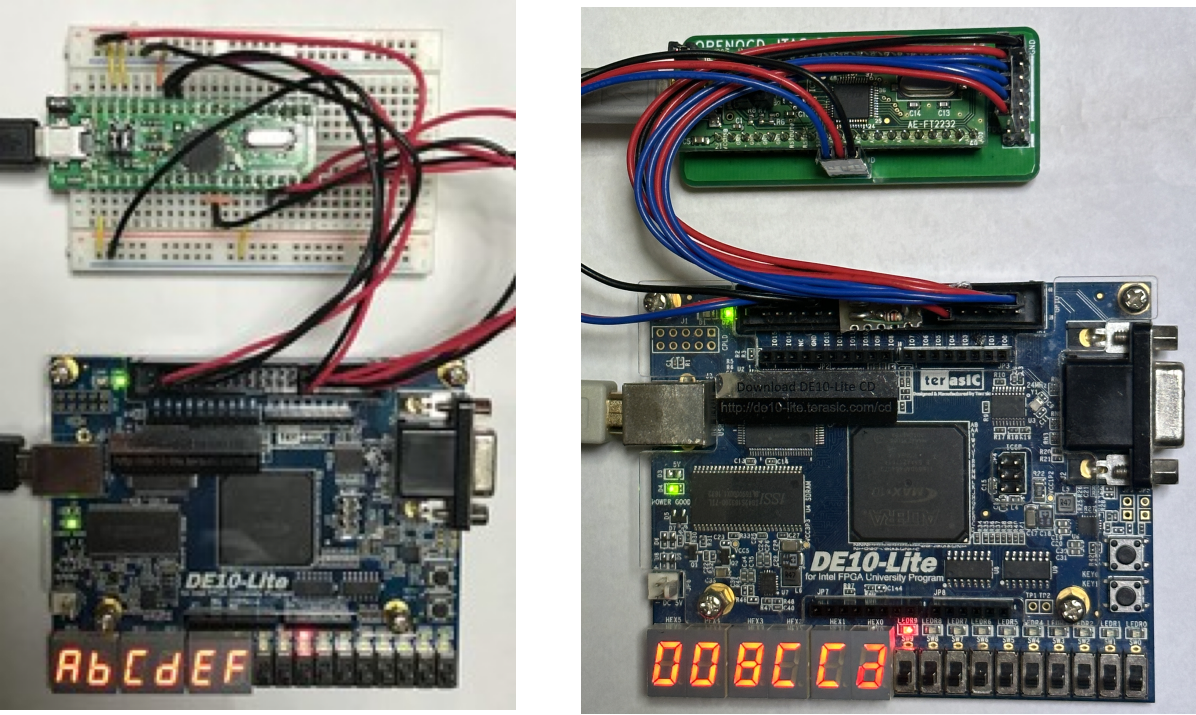
\includegraphics[width=1.0\columnwidth]{./Figure/USB_JTAG_Outline.png}
    \caption{Outline of OpenOCD JTAG/cJTAG Adapter (Left:Breadboard Type, Right:Print Board Type)}
    \label{fig:USBJTAGOUTLINE}
\end{figure}

%=========================================================
\subsection{Schematics of USB to JTAG/cJTAG Interface for OpenOCD}

You can make the interface according to the basic schematic that is shown in Figure \ref{fig:USBJTAGFUNDAMENTAL}. It is recommended to insert resistors of 200 ohms or less between the FT2232D and the FPGA to avoid hardware damage due to signal contention, and to improve signal integrity by reducing cross talk and signal ringing.\\ The detailed schematic including the FT2232D breakout is shown in Figure \ref{fig:USBJTAGSCHEMATICS}.

\begin{figure}[H]
    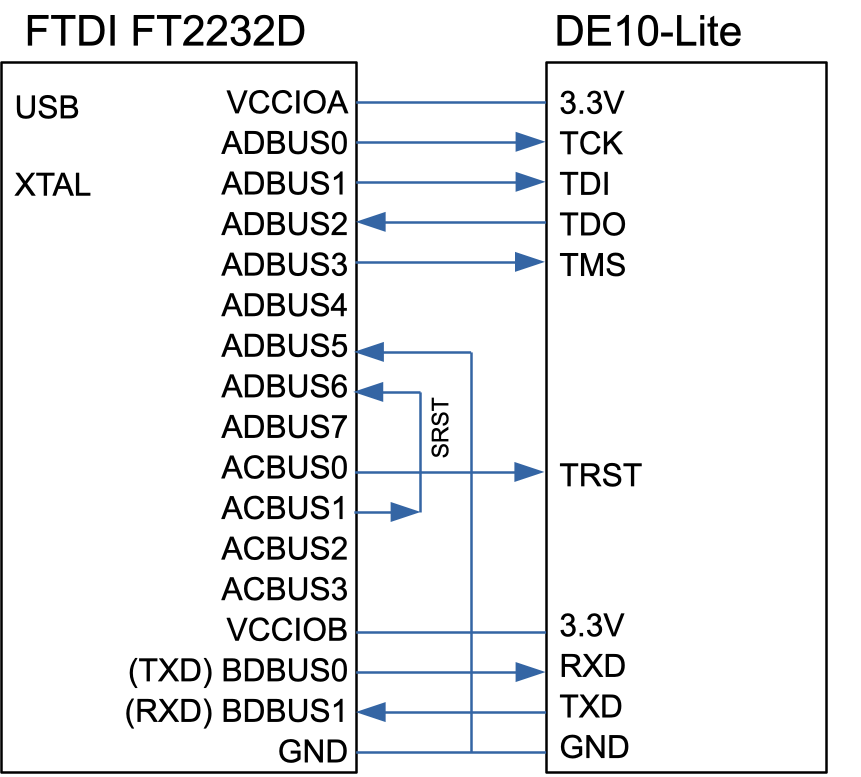
\includegraphics[width=0.75\columnwidth]{./Figure/USB_JTAG_Fundamental.png}
    \caption{Fundamental Connection of OpenOCD JTAG Adapter}
    \label{fig:USBJTAGFUNDAMENTAL}
\end{figure}

\begin{figure}[H]
    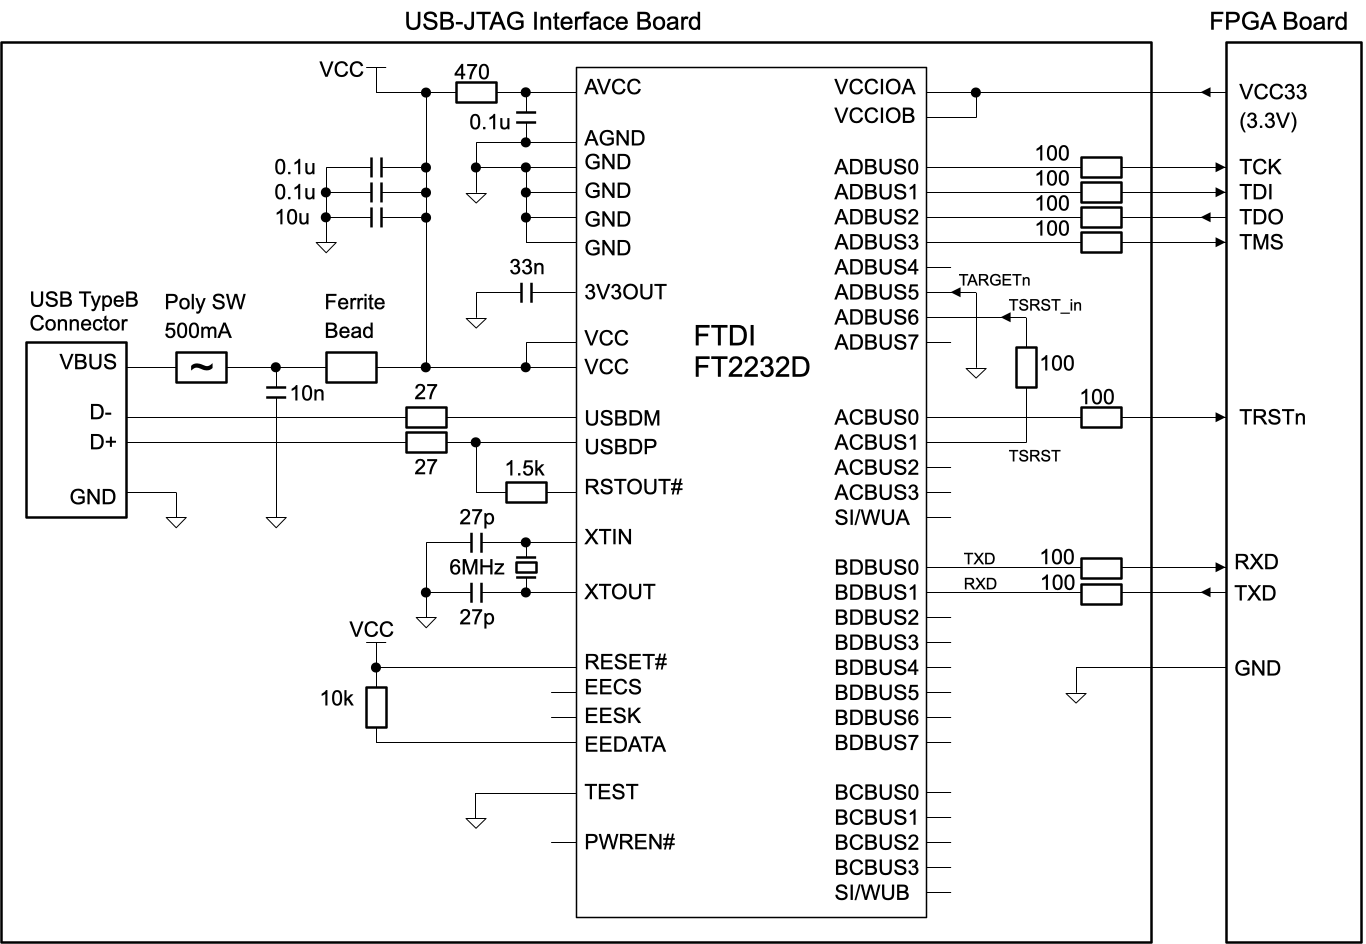
\includegraphics[width=1.0\columnwidth]{./Figure/USB_JTAG_Schematics.png}
    \caption{Detail Schematics of OpenOCD JTAG Adapter}
    \label{fig:USBJTAGSCHEMATICS}
\end{figure}

%=========================================================
\subsection{Connection between USB to JTAG/cJTAG Interface and target FPGA}

Please refer to Figure \ref{fig:USBJTAGCONNECTIONPC} when connecting the JTAG/cJTAG Adapter to the PC in which the OpenOCD works. For this system, the configuration file of OpenOCD is shown in Listing \ref{list:OPENOCDCONFIGPC}.


\begin{figure}[H]
    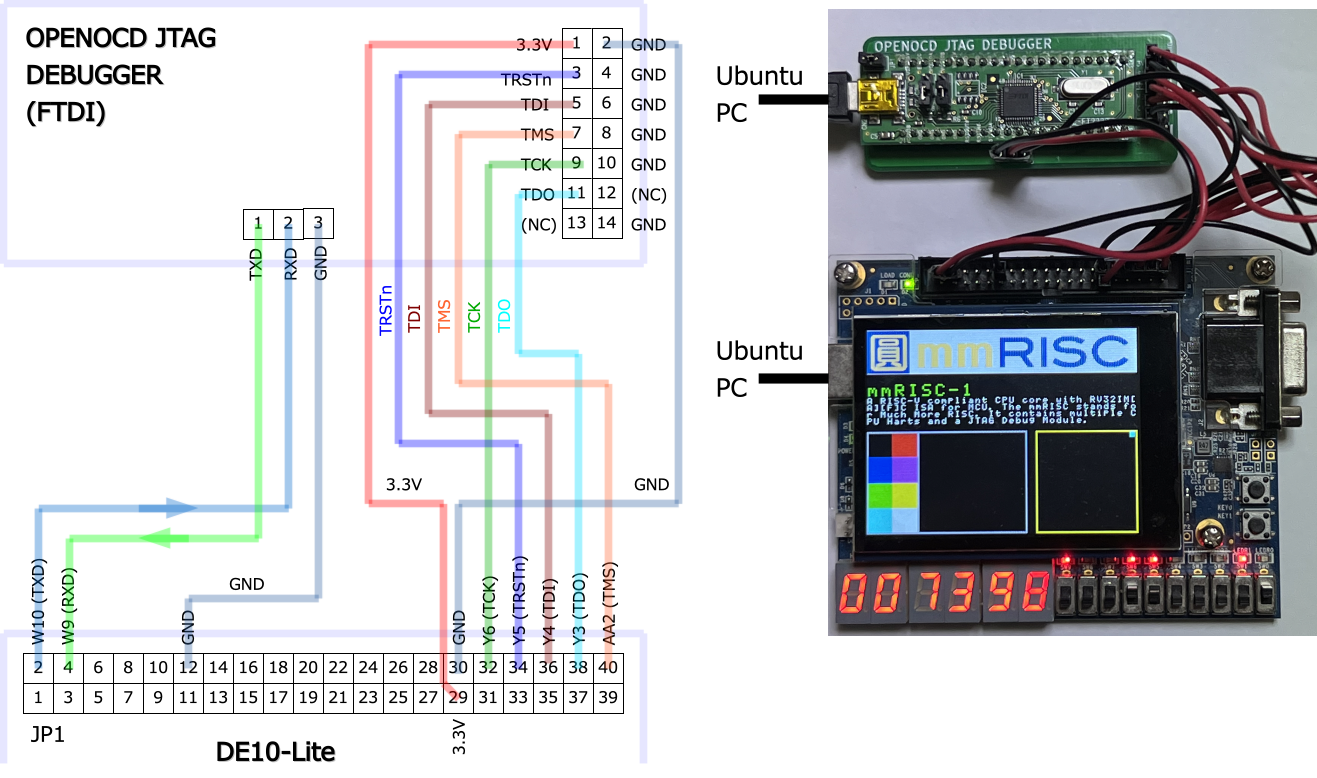
\includegraphics[width=1.0\columnwidth]{./Figure/USB_JTAG_Connection_PC.png}
    \caption{Connection of OpenOCD JTAG Adapter and PC}
    \label{fig:USBJTAGCONNECTIONPC}
\end{figure}

\begin{lstlisting}[caption=OpenOCD Configuration File for Figure \ref{fig:USBJTAGCONNECTIONPC}, label=list:OPENOCDCONFIGPC, captionpos=b,  language=, frame=single, basicstyle=\ttfamily\scriptsize]
adapter driver ftdi
adapter speed 1000
ftdi_device_desc "Dual RS232"
ftdi_vid_pid 0x0403 0x6010

ftdi_layout_init 0x0908 0x0b1b
ftdi_layout_signal nSRST -oe 0x0200
ftdi_layout_signal nTRST -data 0x0100
ftdi_layout_signal LED -data 0x0800

reset_config trst_and_srst

set _chipname riscv
jtag newtap $_chipname cpu -irlen 5

set _targetname $_chipname.cpu
target create $_targetname riscv -endian little -chain-position $_targetname -coreid 0

init

riscv authdata_write 0xbeefcafe
\end{lstlisting}

\textit{NOTE: When you use the commercial Olimex ARM-USB-OCD(H), an example of a corresponding OpenOCD configuration file is shown in Listing \ref{list:OPENOCDCONFIGOLIMEX}.}

\begin{lstlisting}[caption=OpenOCD Configuration File for Olimex ARM-USB-OCD(H), label=list:OPENOCDCONFIGOLIMEX, captionpos=b,  language=, frame=single, basicstyle=\ttfamily\scriptsize]
adapter driver ftdi
adapter speed 1000
ftdi_device_desc "Olimex OpenOCD JTAG ARM-USB-OCD-H"
ftdi_vid_pid 0x15ba 0x002b

ftdi_layout_init 0x0908 0x0b1b
ftdi_layout_signal nSRST -oe 0x0200
ftdi_layout_signal nTRST -data 0x0100
ftdi_layout_signal LED -data 0x0800

reset_config trst_and_srst

set _chipname riscv
jtag newtap $_chipname cpu -irlen 5

set _targetname $_chipname.cpu
target create $_targetname riscv -endian little -chain-position $_targetname -coreid 0

init

riscv authdata_write 0xbeefcafe
\end{lstlisting}


%=========================================================
\subsection{Supplemental Circuit required to use cJTAG}

As described in Section \ref{sec:cJTAG_FPGA}, the FPGA implementation with 2-wire cJTAG requires external pull-up and pull-down resistors on the TMSC pin. In such a case, please make and install a small circuit as shown in Figure \ref{fig:USBCJTAGSUPPLEMENT}.

\begin{figure}[H]
    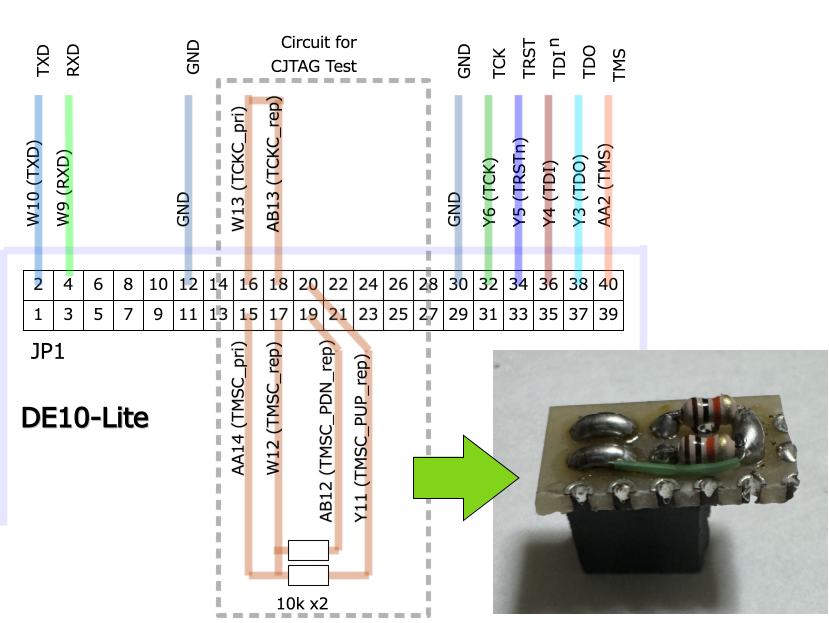
\includegraphics[width=1.0\columnwidth]{./Figure/USB_cJTAG_Supplement.png}
    \caption{Supplement for cJTAG}
    \label{fig:USBCJTAGSUPPLEMENT}
\end{figure}


%=========================================================
\subsection{Raspberry Pi 4 Model B as a Development Environment}

If you have a Raspberry Pi 4 Model B, it can be a comprehensive development environment for RISC-V including mmRISC-1. Please note that the GPIO pins of the Raspberry Pi can be a direct OpenOCD JTAG interface, so you do not need to prepare a dedicated USB to JTAG interface any more. However, the OpenOCD for Raspberry Pi does not support 2-wire compact JTAG (cJTAG) yet, so please configure the FPGA as the mmRISC-1 with the 4-wire JTAG interface.//
You need to install RISC-V development tools on the 64bit Raspberry Pi OS, because the Eclipse requires a 64bit OS. To install all the necessary tools, please follow the steps shown below.\\

(1) Install "Eclipse IDE for Embedded C/C++ Developers" aarch64 version.

(2) Build and Install GNU Tool Chains as follows.

\begin{lstlisting}[language=, frame=single, basicstyle=\ttfamily\scriptsize]
$ sudo apt-get install autoconf automake autotools-dev curl python3             \
              libmpc-dev libmpfr-dev libgmp-dev gawk build-essential bison flex \
              texinfo gperf libtool patchutils bc zlib1g-dev libexpat-dev
$ git clone --recursive https://github.com/riscv-collab/riscv-gnu-toolchain.git
$ ./configure --prefx=/opt/riscv --enable-multilib
$ sudo make
\end{lstlisting}

(3) Install OpenOCD tool as follows. Very simple.

\begin{lstlisting}[language=, frame=single, basicstyle=\ttfamily\scriptsize]
$ sudo apt install openocd
\end{lstlisting}

(4) Download mmRISC-1 resources from Github, and check the OpenOCD Configuration file "mmRISC-1/openocd/openocd\_rpi.cfg" listed in Listing \ref{list:OPENOCDCONFIGRASPI} which configures the Raspberry Pi GPIO as JTAG port as shown in Table \ref{tb:OPENOCDGPIORASPI}. 

(5) Connect the Raspberry Pi to the FPGA board as shown in Figure \ref{fig:USBJTAGCONNECTIONRASPI}.

\begin{lstlisting}[caption=OpenOCD Configuration file for Raspberry Pi, label=list:OPENOCDCONFIGRASPI, captionpos=b,  language=, frame=single, basicstyle=\ttfamily\scriptsize]
adapter driver bcm2835gpio
adapter speed 1000
transport select jtag

#Raspberry Pi 3B/3B+
#bcm2835gpio_peripheral_base 0x3F000000

#Raspberry Pi 4B
bcm2835gpio_peripheral_base 0xFE000000

# Transition delay calculation: SPEED_COEFF/khz - SPEED_OFFSET
# These depend on system clock, calibrated for stock 700MHz
# bcm2835gpio speed SPEED_COEFF SPEED_OFFSET
bcm2835gpio_speed_coeffs 236181 60

# Each of the JTAG lines need a gpio number set: tck tms tdi tdo
# Header pin numbers: 37 29 33 31
bcm2835gpio_jtag_nums 26  5 13  6

# If you define trst or srst, use appropriate reset_config
# Header pin numbers: TRST - 35, SRST - 40
bcm2835gpio_trst_num 19

# reset_config trst_only
bcm2835gpio_srst_num 21

# reset_config srst_only srst_push_pull
# or if you have both connected,
reset_config trst_and_srst srst_push_pull

proc init_targets {} {
    set _CHIPNAME riscv
    jtag newtap $_CHIPNAME cpu -irlen 5

    set _TARGETNAME $_CHIPNAME.cpu
    target create $_TARGETNAME riscv -endian little -chain-position $_TARGETNAME -coreid 0
}
\end{lstlisting}

\begin{table}[H]
    \begin{adjustbox}{scale={0.9}{0.9}}
    \textsf{
    \begin{tabular}{|L{3cm}{3cm}{t}|L{5.5cm}{5.5cm}{t}|L{3cm}{3cm}{t}|L{2.2cm}{2.2cm}{t}|}
        \hline
        %-------------------------------------
        \rowcolor{LightPurple}
        \textbf{BCM2835 GPIO} &
        \textbf{Header Pin No.} &
        \textbf{Signal} &
        \textbf{Note}
        \nextRow \hline
        %-------------------------------------
        GPIO14       & Pin 8          & TXD (output)   & /dev/serial0
        \nextRow \hline
        %-------------------------------------
        GPIO15       & Pin 10         & RXD (input)    & /dev/serial1
        \nextRow \hline
        %-------------------------------------
        GPIO05       & Pin 29         & TMS            & ~
        \nextRow \hline
        %-------------------------------------
        GPIO06       & Pin 31         & TDO            & ~
        \nextRow \hline
        %-------------------------------------
        GPIO13       & Pin 33         & TDI            & ~
        \nextRow \hline
        %-------------------------------------
        GPIO19       & Pin 35         & TRSTn          & ~
        \nextRow \hline
        %-------------------------------------
        GPIO26       & Pin 37         & TCK            & ~
        \nextRow \hline
        %-------------------------------------
        GPIO21       & Pin 40         & SRSTn          & not used
        \nextRow \hline
        %-------------------------------------
        GND          & Pin 6, 9, 14, 20, 25, 30, 34, 39 & GND & ~
        \nextRow \hline
        %-------------------------------------
    \end{tabular}
    }
    \end{adjustbox}
    \caption{Assignments of GPIO of Raspberry Pi 4 Model B as an OpenOCD JTAG Debugger}
    \label{tb:OPENOCDGPIORASPI}
\end{table}

\begin{figure}[H]
    \includegraphics[width=1.0\columnwidth]{./Figure/USB_JTAG_Connection_Raspi.png}
    \caption{Connection of OpenOCD JTAG Adapter and Raspberry Pi}
    \label{fig:USBJTAGCONNECTIONRASPI}
\end{figure}






